\documentclass[12pt]{exam}

\newcommand{\ds}{\ensuremath{\displaystyle}}

\usepackage{amsmath,amsfonts, amsthm}
\usepackage{multicol}
\usepackage{multirow}
\usepackage{harpoon}
\renewcommand{\arraystretch}{1.5}

\newcommand{\harpvec}[1]{\overrightharp{\ensuremath{\mathbf{#1}}}}
\newcommand{\vect}[1]{\harpvec{#1}}
\newcommand{\<}{\langle}
\renewcommand{\>}{\rangle}

% ref: http://pgfplots.sourceforge.net/gallery.html
% ref: http://tex.stackexchange.com/a/74575/79754
\usepackage{pgfplots}% This uses tikz
\pgfplotsset{compat=newest}% use newest version
\tikzset{LineStyle/.style={smooth, ultra thick, samples=400}}

% \printanswers

\begin{document}

\begin{center}
\fbox{\fbox{\parbox{5.5in}{\centering
MATH 1121 - Fall 2015 - Dr. Clontz - Test 3
}}}
\end{center}
\vspace{0.1in}
\makebox[\textwidth]{
  Name:\enspace\hrulefill\hrulefill\hrulefill\space
  Section: MW 1100 (001) / TR 1530 (002)
}

\vspace{12pt}

\begin{itemize}
  \item This test is worth 250 points toward your overall grade.
        Each problem is labeled with its value toward this total. Points
        earned beyond 250 will be counted as bonus.
  \item On multiple choice problems, you do not need to show your work. No
        partial credit will be given.
  \item On full response problems, show all of your work and give a
        complete solution. When in doubt, don't skip any steps. Partial
        credit will be given at the discretion of the instructor.
  \item This exam is open notes, provided that these notes are completely
        in your own handwriting. The professor may take up notes you use
        with your test and return them after the test is graded.
  \item Calculators are not necessary to solve any questions on the test and
        are not allowed.
        Notes on electronic devices must be approved by the instructor
        prior to the test day (e.g. for accomodations) and should be in
        airplane mode.
  \item Tests submitted after the end of 70 minutes will be deducted 25 points,
        with 25 more points deducted every following minute.
\end{itemize}

\newpage

\begin{center}
  \textbf{A few facts from class...}
\end{center}

\noindent
\textbf{Trigonometric function defintions:}
\begin{itemize}
  \item \(\sin\theta = \frac{opp}{hyp}\)
  \item \(\cos\theta = \frac{adj}{hyp}\)
  \item \(\tan\theta = \frac{opp}{adj}=\frac{\sin\theta}{\cos\theta}\)
  \item \(\csc\theta = \frac{hyp}{opp}=\frac{1}{\sin\theta}\)
  \item \(\sec\theta = \frac{hyp}{adj}=\frac{1}{\cos\theta}\)
  \item \(\cot\theta =
    \frac{adj}{opp}=\frac{1}{\tan\theta}=\frac{\cos\theta}{\sin\theta}\)
  \item
Points on the unit circle satisfy \((x,y)=(\cos\theta,\sin\theta)\):
\end{itemize}
\begin{center}
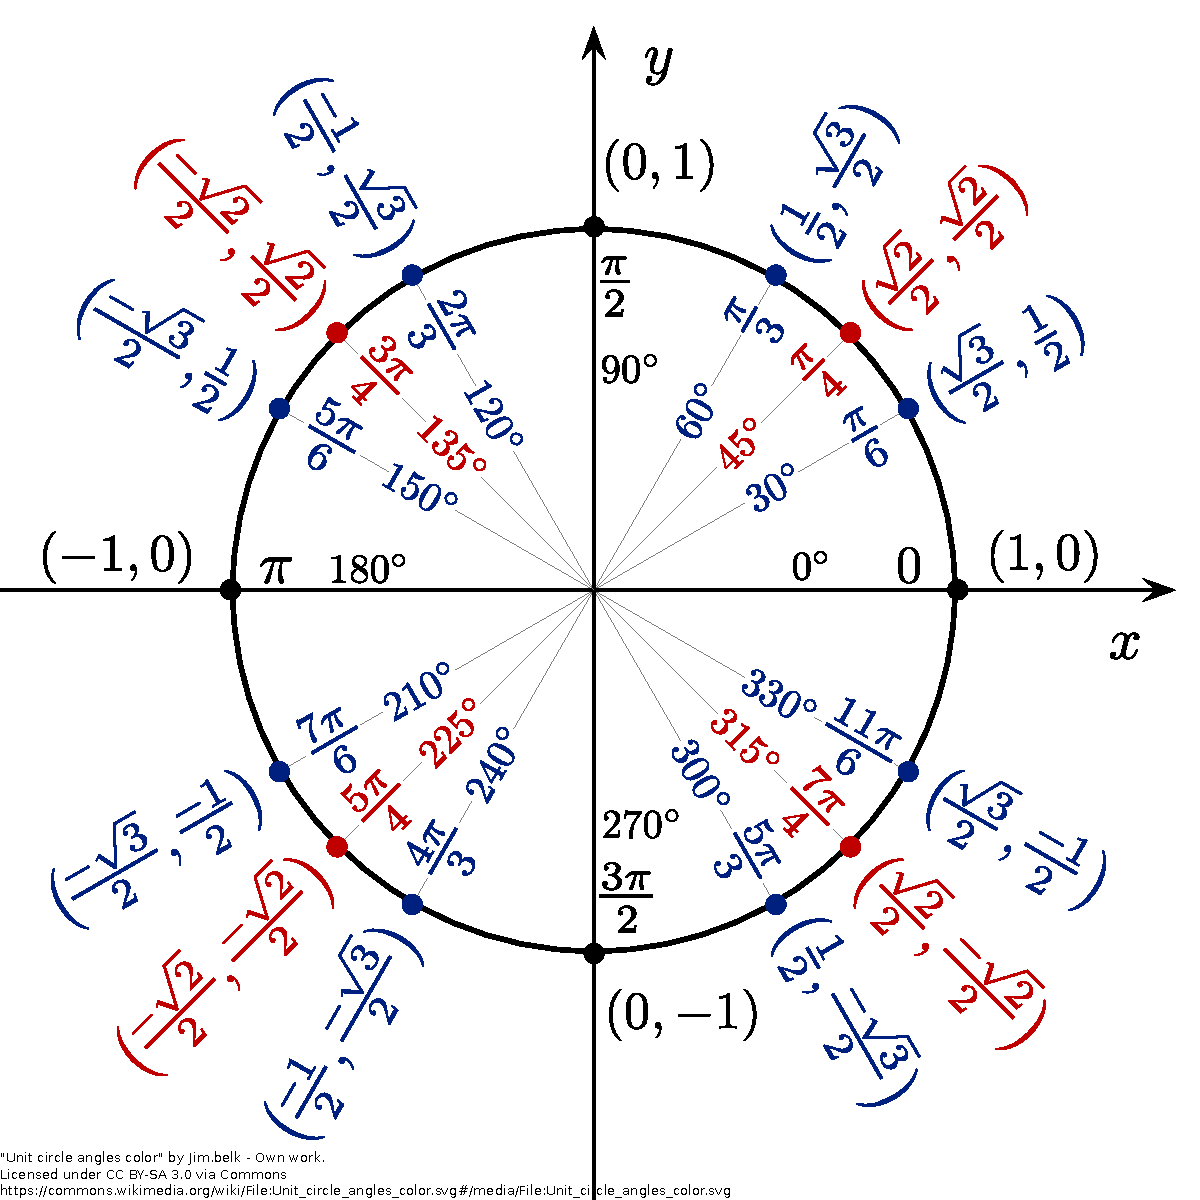
\includegraphics[width=0.7\linewidth]{../unit-circle.pdf}
\end{center}

\noindent
\textbf{Logrithmic Function Definition:}
\begin{itemize}
  \item \(y=\log_b x\) is equivalent to \(x=b^y\)
  \item \(y=\ln x\) is equivalent to \(x=e^y\)
\end{itemize}

\newpage

\noindent
\textbf{Trigonometric/Exponential/Logrithmic Derivatives}

\begin{center}
\begin{tabular}{c|c}
  \(f(x)\) & \(f'(x)\) \\\hline
  \(\sin\theta\) & \(\cos\theta\) \\
  \(\cos\theta\) & \(-\sin\theta\) \\
  \(\tan\theta\) & \(\sec^2\theta\) \\
  \(\cot\theta\) & \(-\csc^2\theta\) \\
  \(\sec\theta\) & \(\sec\theta\tan\theta\) \\
  \(\csc\theta\) & \(-\csc\theta\cot\theta\) \\
  \(\log_b x\) or \(\log_b|x|\) & \(\frac{1}{x}\log_b e\) \\
  \(\ln x\) or \(\ln|x|\) & \(\frac{1}{x}\) \\
  \(b^x\) & \(b^x\ln b\) \\
  \(e^x\) & \(e^x\)
\end{tabular}
\end{center}

\noindent
\textbf{Trigonometric/Exponential/Logrithmic Integrals}

\begin{center}
\begin{tabular}{c|c}
  \(f(x)\) & \(\int f(x)\,dx\) \\\hline
  \(\cos\theta\) & \(\sin\theta+C\) \\
  \(\sin\theta\) & \(-\cos\theta+C\) \\
  \(\sec^2\theta\) & \(\tan\theta+C\) \\
  \(\csc^2\theta\) & \(-\cot\theta+C\) \\
  \(\sec\theta\tan\theta\) & \(\sec\theta+C\) \\
  \(\csc\theta\cot\theta\) & \(-\csc\theta+C\) \\
  \(\frac{1}{x}\) & \(\ln|x|+C\) \\
  \(e^x\) & \(e^x+C\)
\end{tabular}
\end{center}

\newpage

\begin{center}
  \textbf{Multiple Choice (160 points total)}
\end{center}

\begin{questions}

\setcounter{question}{0}

\question[20]
The kinetic energy \(K\) of an object is given by \(K=\frac{1}{2}mv^2\)
where \(m\) is its mass and \(v\) is its velocity?
Which of these expressions represents the rate of change in kinetic energy
with respect to time?

\begin{checkboxes}
  \choice \(0\)
  \choice \(\frac{3}{2}v\)
  \choice \(\frac{1}{2}v^2\frac{dm}{dt}+mv\frac{dv}{dt}\)
  \choice \(2\frac{dm}{dt}\frac{dv}{dt}\)
\end{checkboxes}

\vfill

\question[20]
What is the minimum value of the function \(f(x)=x^2+2x+8\)?

\begin{checkboxes}
  \choice \(f(x)=-2\)
  \choice \(f(x)=4\)
  \choice \(f(x)=7\)
  \choice \(f(x)=10\)
  \choice None of these.
\end{checkboxes}

\vfill

\question[20]
Find \(\int x(x+4)\,dx\).

\begin{checkboxes}
  \choice \(\frac{1}{3}x^3+2x^2+C\)
  \choice \(x^4+4x^3+C\)
  \choice \(2x+C\)
  \choice \(\ln|x+4|+C\)
  \choice None of these.
\end{checkboxes}

\vfill
\newpage

\question[20]
Find \(\int 3x^2\sqrt{x^3+1}\,dx\).

\begin{checkboxes}
  \choice \(\frac{2}{3}(x^3+1)^{3/2}+C\)
  \choice \(\sqrt{3x^2+1}+C\)
  \choice \(\frac{1}{4}x^4+x^3+x+C\)
  \choice \(\frac{x^3}{(3x^2+1)^{1/2}}+C\)
  \choice None of these.
\end{checkboxes}

\vfill

\question[20]
Which of these expressions gives the area bounded above by
the curve \(2x\sqrt{x^2+1}\) and below by the \(x\)-axis between
\(x=0\) and \(x=6\)?


\begin{checkboxes}
  \choice \(\frac{d}{dx}[2x\sqrt{x^2+1}]\)
  \choice \(\tan(2x\sqrt{x^2+1})\)
  \choice \(\int_0^6 2x\sqrt{x^2+1}\,dx\)
  \choice \(e^{2x\sqrt{x^2+1}}\)
  \choice None of these.
\end{checkboxes}

\vfill

\question[20]
Find the derivative \(\frac{dy}{dx}\) of \(y=3\cos(4x)\).

\begin{checkboxes}
  \choice \(3\sec^2(4x)\)
  \choice \(-12\sin(4x)\)
  \choice \(6\csc(4x)\cot(4x)\)
  \choice \(4\sin\cos(4x)\)
  \choice None of these.
\end{checkboxes}

\vfill
\newpage

\question[20]
Find the derivative \(\frac{dy}{dx}\) of \(y=e^{x^2+1}\).

\begin{checkboxes}
  \choice \(2xe^{x^2+1}\)
  \choice \(\ln|x^2+1|\)
  \choice \((x^2+1)e^{2x}\)
  \choice \(\frac{1}{x^2+1}\)
  \choice None of these.
\end{checkboxes}

\vfill

\question[20]
Find \(\ds\int \frac{2x}{3x^2+4}\,dx\).

\begin{checkboxes}
  \choice \(\frac{1}{3}\ln|3x^2+4|+C\)
  \choice \(e^{3x^2+4}+C\)
  \choice \(\frac{1}{2}\sin(3x^2+4)+C\)
  \choice \(x^3+x^2+4x+C\)
  \choice None of these.
\end{checkboxes}

\vfill


\end{questions}




\newpage



\begin{center}
  \textbf{Full Response (100 points total)}
\end{center}

\begin{questions}

\setcounter{question}{8}

\question[20]
  A cylindrical tank with radius \(10\) meters is being filled with water
  at a rate of \(1\) cubic meter per second. How fast is the water rising
  in the tank? Leave your answer in terms of \(\pi\).

  Hint: the formula for the volume of a cylinder is
  \(V=\pi r^2h\) where \(r\) is its radius and \(h\) is its height.

\newpage

\question[20]
  What's the maximum area you can enclose by a rectangle which uses part of
  an existing barn wall for one side and \(200\) feet of
  fencing for the other three sides? (You may assume the barn wall is
  as long as you need.)

\newpage

\question[20]
  Use \(L_4(x)\) where \(f(x)=(8+2x)^{1/2}\) to show that
  \(\sqrt{16.8}\approx 4.1\).

\newpage

\question[20]
  Find a function \(f(x)\) such that \(f'(x)=8x+1\) and
  \(f(-1)=4\).

\newpage

\question[20]
  Find the derivative of \(y=\log_{10}(x^2+1)\).

\end{questions}

\end{document}